\documentclass[12pt,oneside,letterpaper,english]{article}
\usepackage[T1]{fontenc}
\usepackage[latin1]{inputenc}
\usepackage[margin=2.25cm,headheight=26pt,includeheadfoot]{geometry}
\usepackage[english]{babel}
\usepackage{listings}
\usepackage{color}
\usepackage{titlesec}
\usepackage{titling}
\usepackage[framed, numbered]{matlab-prettifier}
\usepackage{changepage}
\usepackage{amsmath}
\usepackage{hyperref}
\usepackage{enumitem}
\usepackage{graphicx}
\usepackage{fancyhdr}
\usepackage{lastpage}
\usepackage{caption}
\usepackage{tocloft}
\usepackage{setspace}
\usepackage{multirow}
\usepackage{titling}
\usepackage{float}
\usepackage{comment}
\usepackage{booktabs}
\usepackage{indentfirst}
\usepackage{lscape}
\usepackage{booktabs,caption}
\usepackage[flushleft]{threeparttable}
\usepackage[english]{nomencl}
\usepackage{xcolor}
\usepackage{lipsum}
\usepackage{datetime2}
\usepackage{natbib}
\usepackage{tabularx}
\usepackage{hyperref}
\usepackage{pdfpages}
% \usepackage{amsmath}       % For math symbols and alignment
% \usepackage{algorithm}     % For algorithm environment
% \usepackage{algorithmicx}  % Algorithm package
% \usepackage{algpseudocode} % For pseudocode formatting
% \usepackage{graphicx}      % For including images
% \usepackage{hyperref}      % For clickable URLs
% \usepackage{listings}      % For listing code if needed

\usepackage{fancyhdr}

\pagestyle{fancy}
\fancyhf{} % Clear all header and footer fields
\rfoot{Page \thepage} % Right footer with "Page X" format

\bibliographystyle{plainnat} 



% --- set footer and header ---
\pagestyle{fancy}
\fancyhf{}

\setlength{\parindent}{2em}
\title{Multiple spliced alignment : a consistency based Approach} % to reference as \title, dont use \maketitle
\makeatletter\let\Title\@title\makeatother



\lstset{language=Matlab,
style=Matlab-editor,
basicstyle=\normalsize\mlttfamily,
numbers=left,
numberstyle={\scriptsize\color{black}},	% size of the numbers
numbersep=0.5cm											
}

\newlist{steps}{enumerate}{1}
\setlist[steps, 1]{leftmargin=1.5cm,label = Step \arabic*:}
\renewcommand{\headrulewidth}{1pt}
\renewcommand{\footrulewidth}{1pt}
\renewcommand{\rmdefault}{ptm}

%\lhead{\Title}
\rhead{\nouppercase{\rightmark}}
\lhead{\Title}
\rfoot{
\includegraphics[height=0.7cm]{figures/241208906_10159878130857049_3729368319539169165_n.png}} % right header logo
\setlength\headheight{16pt}
\setlength{\footskip}{50pt}
\lhead{\Title} %rightH title
\cfoot{\thepage}

% --- End of page settings ---



\begin{document}
\pagenumbering{roman} 

\begin{titlepage}
\begin{center}
\vspace{2cm}
%\textsc{Oregon State University}\\[1.5cm]

\includegraphics[width=0.4\textwidth]{figures/udeslog.png}~\\[1cm]
\vspace{2cm}

% Title
\hrule
\vspace{.5cm}
{ \huge \bfseries Multiple Spliced Alignment : \\ A Consistency Based Approach} % title of the report
\vspace{.5cm}

\hrule
\vspace{1.5cm}

\textsc{\textbf{Author}}\\
\vspace{.5cm}
\centering

% add your name here
Chakirou ALABANI (Group H)\\


\vspace{8cm}

% \centering \today \\ % see latexmkrc for time zone change
\centering BIN702 - Autumn 2024 \\ 
\centering Nadia Tahiri
\end{center}
\end{titlepage}

\newpage
\doublespacing
%\addcontentsline{toc}{section}{Table of Contents}
\renewcommand{\baselinestretch}{1}\normalsize
\tableofcontents
\renewcommand{\baselinestretch}{1}\normalsize
%\singlespacing
\thispagestyle{fancy} % force page style

\newpage
\pagenumbering{arabic} 
\fancyfoot[C]{Page \thepage\ of \pageref{EndOfText}}

\section{Project description}
Alternative splicing is now recognized as a fundamental process in eukaryotic organisms, enabling a single 
gene to generate multiple distinct transcripts. This mechanism affects the majority of human genes 
(\textit{\citep{harrow2006gencode, tress2007implications, kim2008alternative, wang2008alternative, chen2009mechanisms}}) 
and is widely pervasive, playing a crucial role in enhancing the diversity of
the proteome. 
Recent genome-wide studies indicate that 40--60\% of human genes have alternatively spliced forms (\textit{\citep{modrek2002genomic}}). 
This extensive occurrence underscores the need to investigate the evolutionary and conservation patterns of transcript sets, as these 
insights are essential for a deeper understanding of the mechanisms that influence gene evolution.


Understanding the evolution of sets of alternative transcripts is a challenging task and requires automated methods and tools to compare
sets of alternative transcripts from homologous genes. 
Alternative transcripts from homologous genes have traditionally been compared using pairwise spliced 
alignments (PSpAs). A PSpA aligns either a spliced RNA sequence or its DNA equivalent, the coding DNA 
sequence (CDS), with an unspliced DNA sequence. This approach helps identify homologous or corresponding 
exons between sequences, providing crucial insights for genome annotation and gene prediction
(\textit{\citep{stanke2006augustus, dunne2018omgene}}). Various methods have been developed to tackle 
different versions of the PSpA problem, which involves finding the best PSpA between two sequences based 
on a specific optimization function (see \textit{\citep{jammali2019splicedfamalign}}). However, PSpA is limited to 
comparing only two sequences at a time, making it unsuitable for examining the evolution of alternative splicing. 
This restriction also renders it ineffective for analyzing large databases, where multiple sequence comparisons are 
essential.

A logical extension of pairwise spliced alignment (PSpA) for studying the evolution of alternative spliced RNA sets is 
multiple spliced alignment (MSpA). This approach aligns a collection of spliced RNA sequences with their corresponding 
unspliced genomic sequences, allowing for detailed analysis of splicing and exon structures within the gene sequences. 
Unlike traditional multiple sequence alignment (MSA), which focuses solely on sequence similarity, MSpA incorporates the 
splicing and exonic architectures of the input genes. Just as MSA has greatly advanced our understanding of sequence 
evolution, MSpA is anticipated to reveal new insights into the evolution of alternative splicing and the relationships 
among alternative spliced RNA sets.

The MSpA framework also has practical applications for genome annotation by facilitating the identification of exons homologous 
to those in well-characterized species, thereby aiding in the prediction of conserved isoforms in newly annotated genomes.

In the current state of art, there are a few methods available for coomputong MSpAs, with SplicedFamAlignMulti (SFAM) being a 
leading approach (\textit{\citep{jammali2022pairwise}}). SFAM include three extensions : SFAM\_mblock, SFAM\_tcoffee\_p, 
and SFAM\_tcoffee\_m, each providing tailored functionalities for different alignment scenarios. A summary of SFAM methods 
mechanisms is shown in Figure~\ref{fig:spfam-ov}.

\begin{figure}
    \centering
    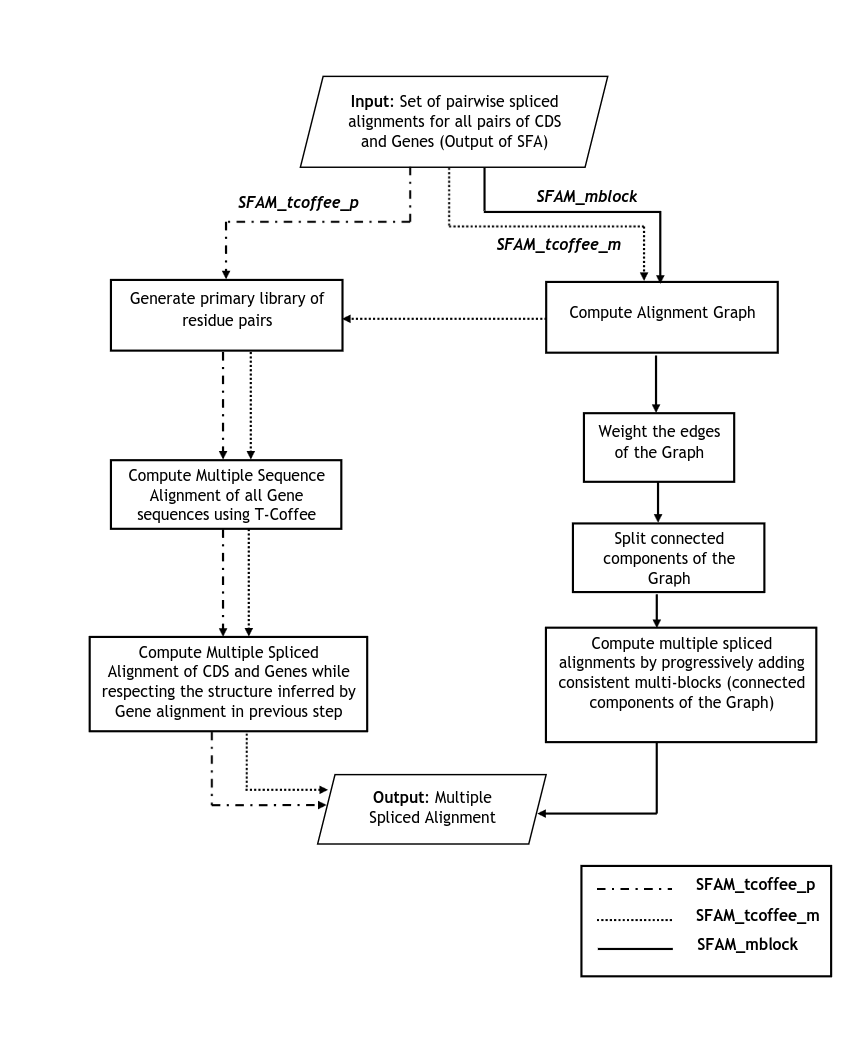
\includegraphics[width=0.3\linewidth]{figures/overview_spFam_methods.png}
    \caption{overview SFAM methods}
    \label{fig:spfam-ov}
\end{figure}

In this report, we present SplicedFamAlignMultiCBA (SFAM\_CBA), a greedy heuristic method developed to merge all 
pairwise spliced alignments (PSpAs) of known coding sequences (CDSs) and gene sequences within a gene family into a 
multiple spliced alignment (MSpA).

 

\section{Materials and methods}
\subsection{Characterization of the MSpA Problem}
\subsubsection{Pairwise Spliced Alignment (PSpA)}
A Pairwise Spliced Alignment (PSpA) refers to the alignment of a Coding Sequence (CDS) with a gene sequence while accounting for the splicing structure. This alignment aims to identify homologous exon sequences and is formulated as a chain of blocks, where each block corresponds to pairwise alignments of segments from both the CDS and gene. 

The significance of PSpA lies in its ability to highlight macroscopic alignments at the splicing level (exon intron structure) rather than at the nucleotide level, emphasizing differences in splicing trends and exon usage across gene families.

\textbf{Definition:} A PSpA consists of blocks, which are conserved segments where both the CDS and gene are included in the alignment. If a CDS is aligned with a gene in a block, it is termed a \textit{conserved block}. Conversely, if only the CDS is included, it is referred to as a \textit{deleted block}.

\subsubsection{Multiple Spliced Alignment (MSpA)}

An MSpA extends the concept of PSpA to include multiple CDSs and gene sequences, facilitating the identification of homologous exons across a broader set of sequences. 

\textbf{Definition:} An MSpA of a set of CDSs \( C \) and genes \( G \) is represented as a chain of multiblocks \( A = \{A[1], \ldots, A[n]\} \). Each multiblock \( A[i] \) includes a key set \( \text{key}(A[i]) \), which is a subset of \( C \cup G \), mapping each sequence to its respective start and end locations \( (s^x_i, e^x_i) \).

The MSpA must satisfy several conditions:
\begin{itemize}
    \item Each multiblock must contain at least one element.
    \item Segments from the same sequence must not overlap across multiblocks.
    \item The segments induced by the MSpA must fully cover the original CDSs.
    \item Segments from aligned genes must be consistent within the same multiblock.
\end{itemize}

\subsubsection{Multiple spliced alignment problem }
\textbf{Input:} A set of CDSs \( C \); a set of genes \( G \), a set of PSpAs \( X = \{ X_{c,g} \mid (c, g) \in C \times G \} \) for all pairs in \( C \times G \).

\textbf{Output:} An MSpA \( A \) of \( C \) on \( G \) that maximizes the sum of the scores of induced PSpAs: \[
\sum_{(c,g) \in C \times G} S(A_{c,g})\] (\textit{\cite{jammali2022pairwise}}).

Several methods are available for computing PSpAs between a gene and a CDS (\textit{\cite{jammali2019splicedfamalign}}).

\subsection{The SFAM-CBA algorithm}
We now present our algorithm for constructing an MSpA for a set of CDSs \( C \) and a set of genes \( G \),
given a set of PSpAs \( X = \{ X_{c,g} \mid (c, g) \in C \times G \} \) for all pairs in \( C \times G \) 
(the MSAPproblem). MSA methods commonly employ greedy heuristics, with the progressive alignment 
strategy (\textit{\cite{feng1987progressive}}) being one of the most widely used approaches.
Distinctively, our method incorporates both the consistency approach and the triplet approach outlined \
in \textit{\cite{t_coffee_alignment}} for pairwise scoring. The consistency-based strategy evaluates how well the alignment of two 
residues or segments in a given pairwise alignment is supported by other precomputed pairwise alignments. Applying this consistency-based 
approach within a progressive alignment allows for the integration of information from all pairwise alignments at each step, 
helping to overcome the typical limitations associated with progressive alignment.

\subsubsection{Boundaries refinement}

Boundary refinement is a crucial step in the consistency based approch for MSpA, aiming to handle overlapping segment matches effectively. 
The refinement algorithm extends the principles established by \textit{Halpern et al. (2002)}, ensuring that all parts of the original segment 
matches can be utilized. 

As described in \textit{\cite{feng1987progressive}}, let \( M = \{M_0, M_1, \ldots, M_{m-1}\} \) represent the set of segment matches, where each match \( M_k = (S_i^{uv}, S_j^{xy}) \) 
consists of segments \( S_i^{uv} \) from sequence \( S_i \) and \( S_j^{xy} \) from sequence \( S_j \). The goal is to refine these segment 
matches into a set of submatches \( M^* = \{M_0^*, M_1^*, \ldots, M_{m'-1}^*\} \) that cover the original matches.

In this context, the refinement process involves ensuring that the set of submatches \( M^* \) satisfies the conditions of tiling the 
original matches:
\[
[u, v - 1] = \bigcup_{M_k' \in M'_*} [u', v' - 1] \quad \text{and} \quad [x, y - 1] = \bigcup_{M_k' \in M'_*} [x', y' - 1].
\]
This ensures that each original match is fully covered by the refined submatches in \( M^* \). 

A resolved set of matches, denoted as \( R \), is desired, where all segments are either disjoint or identical. In such a set, any \( (S_i^{uv}, S_j^{xy}) \in R \) satisfies:
\[
[u, v] \cap \text{supp}_S^i(R) = \{u, v\} \quad \text{and} \quad [x, y] \cap \text{supp}_S^j(R) = \{x, y\}.
\]
The algorithm proceeds to process segment matches sequentially, building a node set \( V_i \) for each sequence \( S_i \), initialized to the support set of the segments. By recursively identifying boundary positions and ensuring necessary cuts are made, the algorithm guarantees a minimum cardinality refinement without introducing superfluous cuts.

% 

\subsubsection{Pairwise Spliced Alignment (PSpA)}

A Pairwise Spliced Alignment (PSpA) refers to the alignment of a Coding Sequence (CDS) with a gene sequence while accounting for the splicing structure. This alignment aims to identify homologous exon sequences and is formulated as a chain of blocks, where each block corresponds to pairwise alignments of segments from both the CDS and gene. 

The significance of PSpA lies in its ability to highlight macroscopic alignments at the splicing level (exon–intron structure) rather than at the nucleotide level, emphasizing differences in splicing trends and exon usage across gene families.

\textbf{Definition:} A PSpA consists of blocks, which are conserved segments where both the CDS and gene are included in the alignment. If a CDS is aligned with a gene in a block, it is termed a \textit{conserved block}. Conversely, if only the CDS is included, it is referred to as a \textit{deleted block}.

\subsubsection{Multiple Spliced Alignment (MSpA)}

An MSpA extends the concept of PSpA to include multiple CDSs and gene sequences, facilitating the identification of homologous exons across a broader set of sequences. 

\textbf{Definition:} An MSpA of a set of CDSs \( C \) and genes \( G \) is represented as a chain of multiblocks \( A = \{A[1], \ldots, A[n]\} \). Each multiblock \( A[i] \) includes a key set \( \text{key}(A[i]) \), which is a subset of \( C \cup G \), mapping each sequence to its respective start and end locations \( (s^x_i, e^x_i) \).

The MSpA must satisfy several conditions:
\begin{itemize}
    \item Each multiblock must contain at least one element.
    \item Segments from the same sequence must not overlap across multiblocks.
    \item The segments induced by the MSpA must fully cover the original CDSs.
    \item Segments from aligned genes must be consistent within the same multiblock.
\end{itemize} 

\subsubsection{Computation of pairwise scores}

The computation of pairwise scores of the set of PSpAs \( X = \{ X_{c,g} \mid (c, g) \in C \times G \} \) is vital for quantifying the similarity between aligned segments of 
sequences. This process relies on the refined segment matches obtained in the previous step. 

Given a set of refined matches \( M^* \), the pairwise score \( S_{ij} \) between sequences \( S_i \) 
and \( S_j \) can be calculated as follows:
\[
S_{ij} = \sum_{k} \text{idty}(M_k^{*}),
\]
where \( \text{idty}(M_k^{*}) \) represents the identity score of the match \( M_k^{*} \) that covers the 
segment \( (S_i^{uv}, S_j^{xy}) \). The identity score can be derived from established scoring matrices 
adjusted for the context of the segments being compared.

To incorporate information from multiple sequences, a weight system can be applied, similar to the one 
discussed by Notredame et al. (1998). By considering intermediate sequences that support the alignment, 
the weights associated with each residue pair are aggregated, enhancing the reliability of the pairwise 
scores. 

The overall weight \( W \) for a pair of aligned residues is computed by examining triplets of sequences 
and accumulating scores based on their alignments. The final weight reflects both the similarity of the 
sequences and their consistency across the dataset, facilitating a more robust alignment process.

\subsubsection{MSpA Computation}

The final stage involves the computation of the multiple sequence alignment (MSA) itself. This process is 
executed through a recursive algorithm that utilizes the refined pairwise scores obtained in the previous 
steps. The goal is to construct an alignment that maximizes the overall score while adhering to the 
constraints imposed by the segment matches.

Let \( T \) represent the phylogenetic tree that organizes the sequences based on their evolutionary 
relationships. The MSpA can be computed recursively as follows:
\[
C(T_i) = \text{Align}(C(T_{\text{left}}), C(T_{\text{right}}), S),
\]
where \( C(T_i) \) is the column list of aligned sequences at node \( T_i \) and \( S \) is the pairwise score matrix derived from the previous computations.

Each internal node of the tree represents an alignment of its child nodes. The alignment function 
\( \text{Align} \) combines the column lists from the left and right child nodes, optimizing the alignment 
based on the accumulated pairwise scores:
\[
\text{Align}(C(T_{\text{left}}), C(T_{\text{right}}), S) = \max_{\text{alignment}} \sum_{\text{pairs}} 
S_{ij},
\]
where the sum is taken over all pairs of aligned segments, and the maximum is computed over all possible 
alignments.

This recursive approach allows the algorithm to build the MSpA incrementally, ensuring that the final 
alignment is optimal with respect to the defined scoring system. The use of a refined weight system 
ensures that the alignment reflects not only the local similarities but also the global relationships 
among all sequences, thereby enhancing the quality and reliability of the MSpA.

A comprehensive and detailed pseudocode of each step in the algorithm is provided in the appendix. 
The implementation of the algorithm, along with the data used, is available on GitHub at 
\textit{https://github.com/chakirouAlabani/BIN702/tree/main/code}. 

\subsection{Experimental setup}
\subsubsection{Dataset}

To assess the performance and demonstrate the utility of SFAM, we used three datasets consisting of 
20 simulated gene families, as well as a dataset of 20 real gene families from the Ensembl 
database (\textit{\cite{zerbino2018ensembl}}). \\ 

\noindent \textit{2.3.1.1 Real dataset} We selected 20 gene families from the Ensembl database, each 
containing genes from six amniote species: human, mouse, dog, dingo, cow, and chicken. For each family, 
only the genes from these six species were retained, and the dataset includes their sequences and all 
corresponding CDSs. CDS sets for each gene family were obtained from Ensembl releases 97 and 98, as 
release 98 introduced an updated gene annotation for dog, resulting in an increase from 19,857 to 20,257 
coding genes and from 39,074 to 60,994 transcripts. This dataset was used to assess the ability of 
SpliceFamAlignMulti to predict the new dog CDSs added in release 98, based on spliced alignments 
calculated from release 97 data. Table~\ref{tab:real_dataset} (\textit{\cite{jammali2022pairwise}}) provides a detailed description of this real dataset. \\


\begin{table}[h!]
\centering
\begin{tabularx}{\textwidth}{|l|c|X|c|X|c|}
    \hline
Gene family (tree) ID & No. of total genes & No. of total CDS (97\-98) & No. of dog genes & No. of dog CDS (97\-98) & PID \\
\hline
ENSGT00390000063205 & 19 & 42\-45 & 3 & 3\-6 & 0.098 \\
ENSGT00390000008371 & 12 & 27\-28 & 2 & 2\-3 & 0.604 \\
ENSGT00390000000715 & 6 & 12\-15 & 1 & 1\-4 & 0.474 \\
ENSGT00940000157909 & 6 & 31\-35 & 1 & 1\-5 & 0.623 \\
ENSGT00530000063187 & 17 & 28\-30 & 3 & 3\-5 & 0.177 \\
ENSGT00950000182978 & 24 & 88\-103 & 4 & 4\-19 & 0.106 \\
ENSGT00950000182681 & 43 & 79\-89 & 7 & 9\-19 & 0.147 \\
ENSGT00950000182875 & 37 & 33\-67 & 6 & 4\-10 & 0.112 \\
ENSGT00950000182728 & 35 & 75\-83 & 6 & 6\-14 & 0.073 \\
ENSGT00950000182931 & 24 & 46\-57 & 4 & 4\-8 & 0.168 \\
ENSGT00950000182705 & 39 & 111\-115 & 5 & 5\-9 & 0.087 \\
ENSGT00390000063023 & 23 & 41\-46 & 4 & 6\-11 & 0.103 \\
ENSGT00940000153241 & 14 & 16\-19 & 3 & 3\-6 & 0.06 \\
ENSGT00950000182956 & 23 & 56\-71 & 4 & 5\-20 & 0.257 \\
ENSGT00950000182783 & 29 & 72\-77 & 4 & 4\-9 & 0.045 \\
ENSGT00950000183192 & 8 & 69\-72 & 3 & 3\-6 & 0.051 \\
ENSGT00950000182727 & 24 & 73\-84 & 5 & 6\-17 & 0.047 \\
ENSGT00390000004965 & 7 & 7\-8 & 1 & 1\-2 & 0.89 \\
ENSGT00390000003967 & 6 & 9\-12 & 1 & 1\-2 & 0.792 \\
ENSGT00390000005532 & 6 & 12\-13 & 1 & 1\-2 & 0.545 \\
\hline
\end{tabularx}
\caption{Description of the real dataset of 20 gene families (PID)}
\label{tab:real_dataset}
\end{table}


\noindent \textit{2.3.1.2 Simulated data} Since true MSpAs of real gene families were unavailable for validation, we generated three 
datasets of 20 simulated gene families with gene sequences and CDSs using SimSpliceEvol (Kuitche et al., 2019). SimSpliceEvol simulates 
the evolution of gene splicing structures and transcript sets through alternative splicing events. Starting with a gene tree with 
evolutionary rates represented by branch lengths, it uses distributions from 189 eukaryotic species to model exon and intron lengths, 
alternative transcript numbers, and exon counts per gene.

The simulation begins with an ancestral gene sequence with exon intron structure and associated CDSs at the root of the tree, 
which evolves along the branches to produce gene sequences and CDSs for each node. The model simulates two levels of evolution: 
gene level changes, such as exon duplication, gain, loss, and sequence mutations in exonic (coding) and intronic (noncoding) regions, 
and transcript-level changes, including the creation, loss, and modification of isoforms via alternative splicing.

We generated three datasets: (1) "Small" with low evolutionary rates on a tree of five primates, (2) "Medium" with moderate rates using a 
tree of five primates and rodents, and (3) "Large" with high rates using a tree of five amniote species. The gene trees used in these 
simulations, obtained from the Ensembl Compara database (Zerbino et al., 2018), are described in Supplementary Material. SimSpliceEvol 
also provides the true MSA of all CDS and gene sequences and identifies groups of splicing orthologs. These groups consist of CDSs 
that evolved from a common ancestral CDS without alternative splicing events. Table~\ref{tab:simulated_datasets} (\textit{\cite{jammali2022pairwise}}) provides further details on the simulated datasets.

\begin{table}[h!]
    \centering
    \begin{tabular}{lccc}
    \hline
     & \textbf{Small} & \textbf{Medium} & \textbf{Large} \\
    \hline
    Number of families & 20 & 20 & 20 \\
    Number of genes per family & 5 & 5 & 5 \\
    Avg. number of CDS & 8.8 & 8.55 & 9.35 \\
     & (3.02) & (3.04) & (2.70) \\
    Avg. CDS length & 802.65 & 820.49 & 778.13 \\
     & (204.41) & (288.37) & (281.77) \\
    Avg. gene length & 2358.71 & 2724.82 & 2418.22 \\
     & (713.76) & (813.09) & (601.44) \\
    Avg. pairwise PID (\%) & 71.24 & 54.39 & 41.61 \\
     & (4.36) & (2.52) & (2.4) \\
    \hline
    \end{tabular}
    \caption{Summary of simulated datasets.}
    \label{tab:simulated_datasets}
\end{table}

\subsubsection{Evaluated methods}
To the best of our knowledge, SFAM-CBA has no direct competitors for MSpA, aside from the original SFAM method. Therefore, 
the performance of SFAM-CBA algorithms will be compared against the three SFAM extensions (SFAM\_mblock, SFAM\_tcoffee\_p, and SFAM\_tcoffee\_m) 
as well as other popular multiple sequence alignment (MSA) methods, using the resulting multiple CDS alignments. This comparison 
is relevant because the quality of a multiple CDS alignment induced by an MSpA is closely linked to the overall quality of the MSpA itself. \\
    

\noindent \textbf{\textit{MSA methods}} SFAM-CBA was compared with widely used MSA methods, including \textit{MUSCLE} \citep{edgar2004}, 
\textit{MAFFT} \citep{katoh2013}, \textit{MACSE} \citep{ranwez2018}, \textit{CLUSTAL\_O} \citep{sievers2011}, \textit{PRANK} 
\citep{loytynoja2005, loytynoja2008}, \textit{T-Coffee} \citep{notredame2000}, and \textit{Mirage} \citep{nord2018}. \textit{MUSCLE} 
uses a log-expectation scoring system to accelerate its progressive alignment process. \textit{MAFFT} identifies homologous regions 
using the fast Fourier transform to improve alignment efficiency. \textit{MACSE} is specifically designed for coding sequences and 
accounts for the codon structure, making it ideal for aligning protein-coding nucleotide sequences. \textit{CLUSTAL\_O} utilizes 
guide trees and a profile-profile comparison based on hidden Markov models to generate MSAs. \textit{PRANK} is a probabilistic 
alignment tool that uses maximum likelihood estimation, incorporating evolutionary distances between sequences. \textit{T-Coffee} 
employs a consistency-based progressive alignment strategy, leveraging a library of pairwise residue matches obtained from initial 
pairwise alignments. \textit{Mirage} focuses on aligning alternatively spliced protein isoforms by mapping protein sequences to their 
genomic counterparts and aligning based on these mappings.

\subsubsection{Performance metrics}
Based on the true MSAs of the CDSs for each gene family in the simulated datasets, we calculated the precision, recall, F-score, 
and computation time for each method and each gene family. \textit{Precision} is defined as the proportion of nucleotide pairs in the predicted 
alignment that also appear in the true alignment. \textit{Recall} represents the proportion of nucleotide pairs in the true alignment that are also 
found in the predicted alignment. The \textit{F-score} is the harmonic mean of precision and recall, providing a balanced measure of both.

To account for the fact that SFAM-CBA and Mirage use the gene sequences as guides to enhance the alignment of CDSs, we evaluated two 
sets of results. The first set was obtained by aligning only the CDSs directly with other MSA methods (MUSCLE, MAFFT, MACSE, CLUSTAL\_O, 
PRANK, T-Coffee). The second set of results was was produced by aligning both gene sequences and CDSs with these MSA tools 
(referred to as \textit{MUSCLE\_G}, \textit{MAFFT\_G}, \textit{MACSE\_G}, \textit{CLUSTAL\_O\_G}, \textit{PRANK\_G}, \textit{T-Coffee\_G}), 
and then extracting the CDS alignments from the full gene MSAs. For both sets of results, we computed precision, recall, F-score, and 
computing time. For \textit{SFAM-CBA}, the total computing time includes the time required for generating pairwise spliced alignments (PSpAs).


\label{EndOfText}

\newpage
% \pagenumbering{Roman} 
\pagenumbering{gobble}
\addcontentsline{toc}{section}{List of Figures}
\fancyfoot[C]{Page \thepage\ of \pageref{endOfDoc}}
\listoffigures
% \thispagestyle{fancy}

\newpage
\addcontentsline{toc}{section}{List of Tables}
\listoftables
% \thispagestyle{fancy}
% \thispagestyle{fancy}
\newpage
\pagenumbering{gobble}
\addcontentsline{toc}{section}{References}
% \bibliography{} 
\bibliography{document}
% \bibliographystyle{plainnat}
% \thispagestyle{fancy}

\newpage
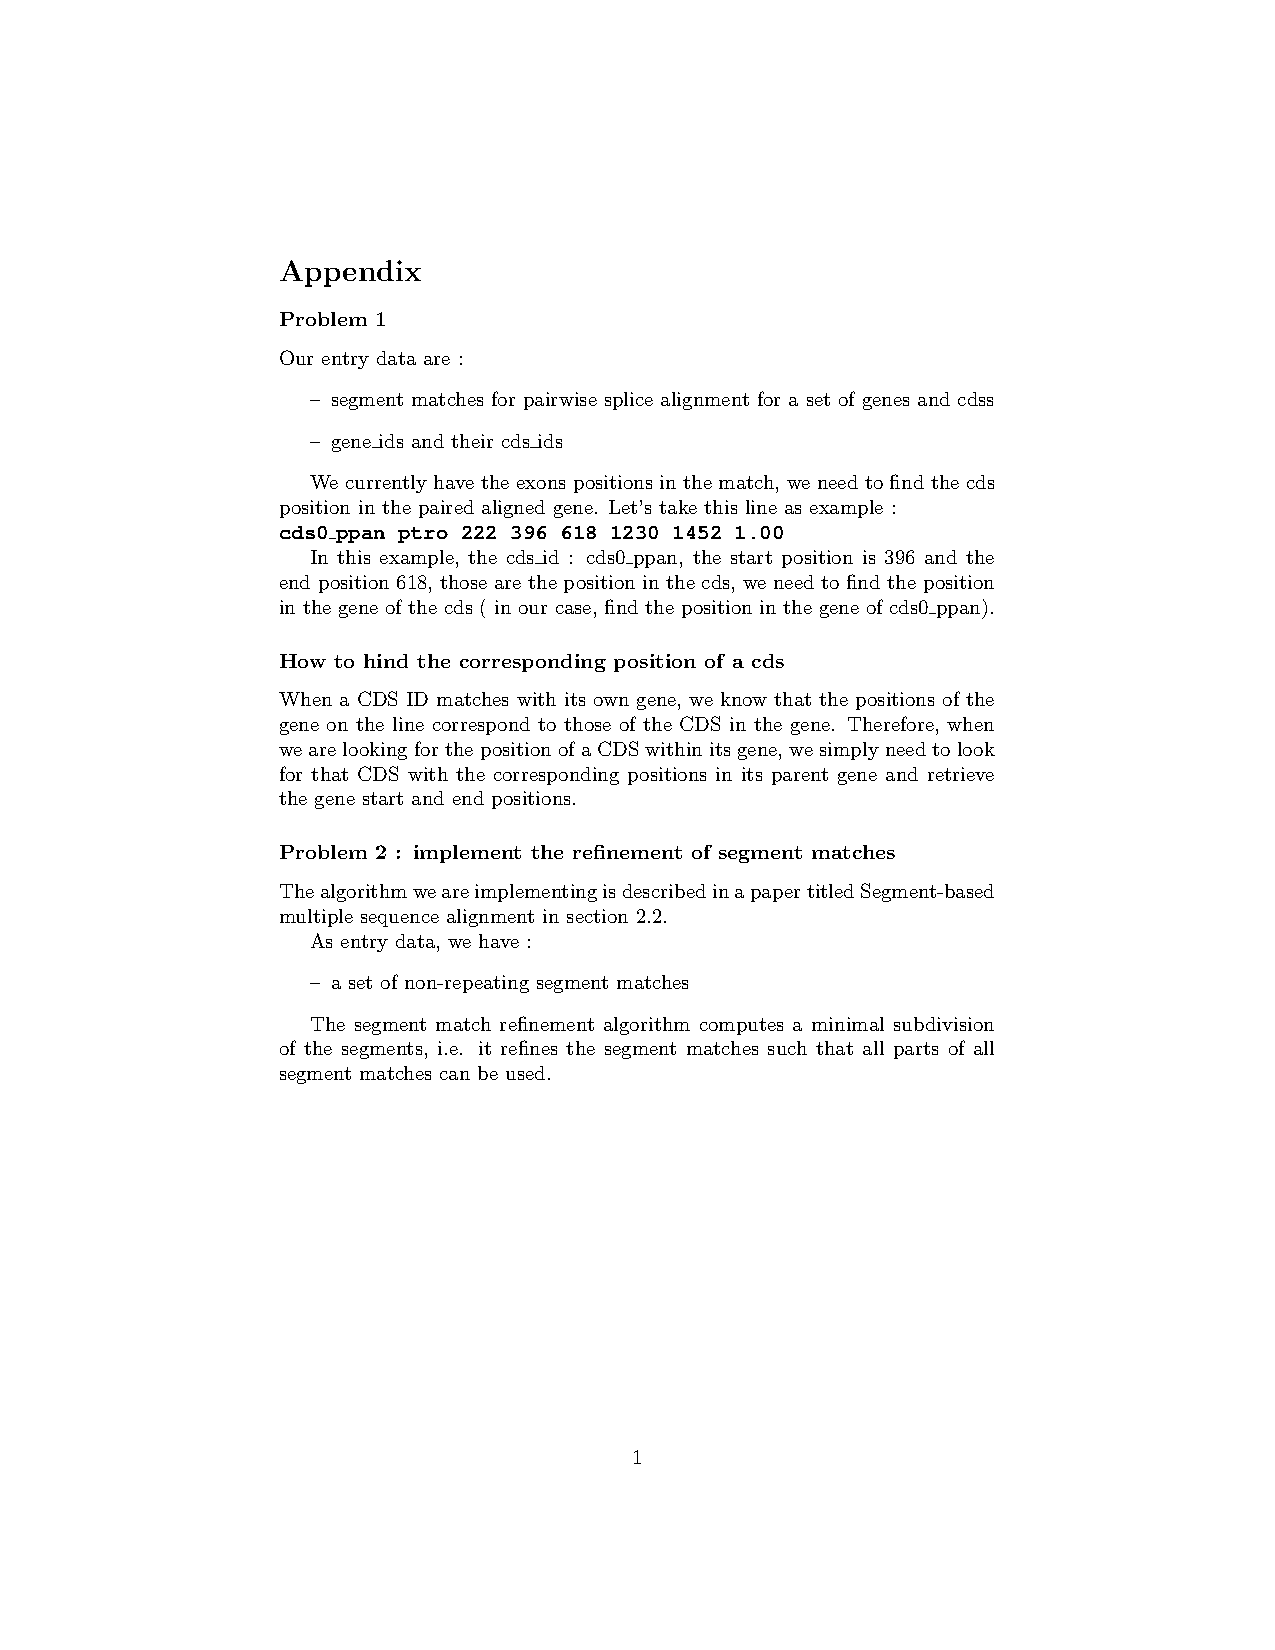
\includepdf[pages=-]{sources/appendix2a.pdf}

% \section{Appendix}
% \subsection*{Problems \& algos}
% \subsubsection*{Problem 1}
%     Our entry data are : 
%     \begin{itemize}
%         \item[--] segment matches for pairwise splice alignment for a set of genes and cdss
%         \item[--] gene\_ids and their cds\_ids
%     \end{itemize}

%     We currently have the exons positions in the match, we need to find the cds position in the paired aligned gene. Let's take this line as example : 
    
%     \noindent\textbf{\texttt{cds0\_ppan	ptro	222	396	618	1230	1452	1.00 }}

%     In this example, the cds\_id : cds0\_ppan, the start position is 396 and the end position 618, those are the position in the cds, we need to find the position in the gene of the cds ( in our case, find the position in the gene of cds0\_ppan). 

% \subsubsection*{Algo 1}
    
% \begin{algorithm}
%     \caption{Retrieve the position of the aligned exon in the other gene of the alignment}
%     \begin{algorithmic}[1]
%         \STATE \textbf{Input:} 
%         \STATE \quad $data$: segment matches for pairwise splice alignment for a set of genes and cdss
%         \STATE \quad $source\_to\_target\_file\_path$: gene\_ids and their cds\_ids
        
%         \STATE \textbf{Output:} 
%         \STATE \quad $processed$: A dictionary with additional exon position information added to the alignment data
        
%         \Procedure{FindExonPosInPairedGene}{$data, source\_to\_target\_file\_path$}
%             \STATE $cds\_gene\_map \gets \text{get\_cds\_gene\_map}(source\_to\_target\_file\_path)$
%             \STATE $result \gets \{ []\}$
            
%             \FOR{\textbf{each} $key, values$ \textbf{in} $data$}
%                 \FOR{\textbf{each} $match$ \textbf{in} $values$}
%                     \STATE $cdsId \gets match[0]$
%                     \STATE $gene_b \gets match[1]$
%                     \STATE $gene_a \gets cds\_gene\_map[cdsId]$
%                     \STATE $search\_key \gets \text{concatenate}(cdsId, gene_a)$
                    
%                     \IF{$gene_a \neq gene_b$}
%                         \STATE $result \gets \text{search\_exon\_pos\_in\_pair\_aligned\_gene}(data[search\_key], [match[3], match[4]], \text{line\_length}=10)$
                        
%                         \IF{$\text{length}(result) == 1$}
%                             \STATE \text{append}(result[0][5], result[0][6]) \text{to} match
%                             \STATE $formatted\_match \gets \text{iteration\_result\_to\_refinement\_entry\_format\_file}(match, cds\_gene\_map)$
%                             \STATE \text{append}(formatted\_match) \text{to} processed['all']
%                         \ELSE
%                             \STATE \text{append}("-", "-") \text{to} match
%                         \ENDIF
%                     \ELSE
%                         \STATE \text{append}("-", "-") \text{to} match
%                     \ENDIF
%                 \ENDFOR
%             \ENDFOR
        
%             \STATE \RETURN $processed$
%         \EndProcedure
%     \end{algorithmic}
% \end{algorithm}

% \subsubsection*{How to hind the corresponding position of a cds}

% When a CDS ID matches with its own gene, we know that the positions of the gene on the line correspond to those of the CDS in the gene. Therefore, when we are looking for the position of a CDS within its gene, we simply need to look for that CDS with the corresponding positions in its parent gene and retrieve the gene start and end positions.


% \begin{algorithm}
%     \caption{Search Exon Positions in a Pair of Aligned Genes}
%     \begin{algorithmic}[1.1]
%         \STATE \textbf{Input:} 
%         \STATE \quad $data$: List of lines to search through
%         \STATE \quad $cds\_segment$: Tuple containing the start and end positions of the exon
%         \STATE \quad $line\_length$: Minimum length of the line to consider (default is 8)
        
%         \STATE \textbf{Output:} 
%         \STATE \quad $result$: List of lines that match the search criteria based on the exon positions
        
%         \Procedure{search\_exon\_pos\_in\_pair\_aligned\_gene}{$data, cds\_segment, line\_length=8$}
%             \STATE $(cds\_start, cds\_end) \gets cds\_segment$
%             \STATE $cds\_start \gets \text{int}(cds\_start)$
%             \STATE $cds\_end \gets \text{int}(cds\_end)$
%             \STATE $result \gets []$
            
%             \FOR{\textbf{each} $line$ \textbf{in} $data$}
%                 \IF{$( \text{int}(line[3]) == \text{exonStart} \land \text{int}(line[4]) == \text{exonEnd}) $}
%                     \STATE \text{append} $line$ \text{to} $result$
%                 \ENDIF
%             \ENDFOR

        
%             \STATE \RETURN $result$
%         \EndProcedure
%     \end{algorithmic}
% \end{algorithm}
    
% \subsubsection*{Problem 2 : implement the refinement of segment matches}

% The algorithm we are implementing is described in a paper titled \href{https://academic.oup.com/bioinformatics/article/24/16/i187/200409}{Segment-based multiple sequence alignment} in section 2.2.

% As entry data, we have : 
%     \begin{itemize}
%         \item[--] a set of non-repeating segment matches
%         % \item[--] 
%     \end{itemize}


%  The segment match refinement algorithm computes a minimal subdivision of the segments, i.e. it refines the segment matches such that all parts of all segment matches can be used \cite{10.1093/bioinformatics/btn281}.


% \begin{algorithm}
% \caption{mult\_seg\_match\_refinement}
%     \begin{algorithmic}[2.1]
%         \REQUIRE file\_path: string
%         \ENSURE refined multi-segment matches
%         % \IF{file\_path is empty}
%         %     \PRINT{Error: File path cannot be empty}
%         %     \RETURN
%         % \ENDIF
%         % \STATE output $\gets$ \texttt{get\_output\_folder(OUTPUT\_FOLDER)} + \texttt{get\_family(file\_path).replace('\_extended\_', '')} + "\_output.txt"
%         % \STATE original\_data $\gets$ \texttt{file\_to\_list(file\_path)}
%         \STATE segment\_matches $\gets$ \texttt{original\_data[2:]}
%         \STATE Vi $\gets$ \texttt{build\_Vi(segment\_matches)}
%         \STATE \texttt{del\_duplicates\_sort\_Vi(Vi)}
%         \STATE \texttt{visualize\_Vi(Vi, output)}
%         \STATE Ti $\gets$ \texttt{build\_Ti(segment\_matches)}
%         \FORALL{match in segment\_matches}
%             % \IF{match is empty}
%             %     \CONTINUE
%             % \ENDIF
%             \STATE boundaries $\gets$ \texttt{get\_match\_boundaries(match)}
%             \FORALL{w in boundaries}
%                 \STATE gene1 $\gets$ \texttt{gene\_of\_boundary(index, match)}
%                 \STATE Vi $\gets$ \texttt{refine(w, Ti, Vi, gene1)}
%             \ENDFOR
%         \ENDFOR
%         \STATE \texttt{del\_duplicates\_sort\_Vi(Vi)}
%         \STATE \texttt{visualize\_Vi(Vi, output, True)}
%         \PRINT{Refinement output path : \texttt{output}}
%         \RETURN Vi
%     \end{algorithmic}
% \end{algorithm}


% \begin{algorithm}
%     \caption{refine}
%     \begin{algorithmic}[1]
%         \REQUIRE $w$, $Ti$, $Vi$, $gene1$
%         \ENSURE Refined $Vi$
%         \STATE $stack \gets [(w, gene1)]$
%         \WHILE{$stack \neq []$}
%             \STATE $(current\_w, current\_gene1) \gets stack.pop()$
%             \STATE $overlaps \gets get\_overlaps(Ti, current\_w, current\_gene1)$
%             \FORALL{$lq \in overlaps$}
%                 \IF{$lq[0].data == current\_gene1[\text{"gene\_id"}]$}
%                     \STATE $(u, v, u\_v\_gene) \gets (lq[0].begin, lq[0].end, lq[0].data)$
%                     \STATE $(x, y, x\_y\_gene) \gets (lq[1].begin, lq[1].end, lq[1].data)$
%                 \ELSE
%                     \STATE $(u, v, u\_v\_gene) \gets (lq[1].begin, lq[1].end, lq[1].data)$
%                     \STATE $(x, y, x\_y\_gene) \gets (lq[0].begin, lq[0].end, lq[0].data)$
%                 \ENDIF
%                 \STATE $h \gets x + (current\_w - u)$
%                 \STATE $gene2\_id \gets x\_y\_gene$
%                 \STATE $consider\_h \gets x < h < y$
%                 \STATE $gene2 \gets \{ \text{"gene\_id"}: gene2\_id, \text{"u"}: u, \text{"v"}: h \}$
%                 \IF{$consider\_h$}
%                     \IF{$gene2\_id \notin Vi$}
%                         \STATE $Vi[gene2\_id] \gets []$
%                     \ENDIF
%                     \IF{$h \notin Vi[gene2\_id]$}
%                         \STATE $Vi[gene2\_id].append(h)$
%                         \STATE $stack.append((h, gene2))$
%                     \ENDIF
%                 \ENDIF
%             \ENDFOR
%         \ENDWHILE
%         \STATE \RETURN $Vi$
%     \end{algorithmic}
% \end{algorithm}

% \subsubsection*{Problem 3 : alignment graph}

% The algorithm we are implementing is described in the same paper in section 2.1. The purpose of this algo is to construct an alignment graph from refined segment matches for genes. 

% \subsubsection*{Overall steps of the algorithm}
% \begin{enumerate}
%     \item Build vertices from the refined segments for each gene. A vertex is a tuple size 3:
%     \begin{enumerate}
%         \item[0] gene id
%         \item[1] start position
%         \item[2] length
%     \end{enumerate}
%     \item Build edges from vertices.
%     \begin{enumerate}
%         \item An edge exists if there is a match between the 2 vertices.
%         \begin{itemize}
%             \item $\diamond$ start\_i == start\_j
%             \item $\diamond$ length\_i == length\_j
%         \end{itemize}
%         \item The weight of the edge is found using the percent identity (PI) of the match represented by the edge. The triplet approach is the way:
%         \begin{enumerate}
%             \item Compute edge percent identity.
%             \item Calculate the weight (triplet approach).
%         \end{enumerate}
%     \end{enumerate}
%     \item Generate the graph using the edges.
%     \begin{itemize}
%         \item The edge structure (tuple):
%         \begin{enumerate}
%             \item[0] Vertex origin
%             \item[1] Vertex target
%             \item[2] Weight
%         \end{enumerate}
%     \end{itemize}
% \end{enumerate}

% \begin{algorithm}
%     \caption{build\_alignment\_graph}
%     \begin{algorithmic}[3.1]
%         \REQUIRE Refined segment matches for genes
%         \ENSURE Alignment graph
%         \STATE $vertices \gets build\_vertices(V_i)$
%         \STATE $edges \gets build\_edges(vertices)$
%         \FORALL{vertex \textbf{in} $vertices$}
%             \STATE Get weighted edges using vertices
%             \STATE Get trace from weighted edges
%         \ENDFOR
%         \STATE $build\_graph$
%     \end{algorithmic}
% \end{algorithm}

% \begin{algorithm}
%     \caption{build\_vertices}
%     \begin{algorithmic}[1]
%         \REQUIRE $Vi$ 
%         \ENSURE $vertices$
%         \STATE $vertices \gets []$
%         \FORALL{$(gene\_id, boundaries) \in Vi$}
%             \FOR{$index \gets 0$ \textbf{to} $len(boundaries) - 2$}
%                 \STATE $boundary \gets boundaries[index]$
%                 \STATE $next\_boundary \gets boundaries[index + 1]$
%                 \STATE $start\_boundary \gets \text{int}(boundary)$
%                 \STATE $segment\_length \gets \text{int}(next\_boundary) - start\_boundary$
%                 \STATE $vertex \gets (gene\_id, start\_boundary, segment\_length)$
%                 \STATE $vertices.append(vertex)$
%             \ENDFOR
%         \ENDFOR
%         \STATE \RETURN $vertices$
%     \end{algorithmic}
% \end{algorithm}
        
% \begin{algorithm}
%     \caption{build\_edges}
%     \begin{algorithmic}[3.2]
%         \REQUIRE $vertices$, $target\_data$
%         \ENSURE $edges$
%         \STATE $edges \gets []$
%         \STATE $weightless\_edges \gets []$
%         \FOR{$i \gets 0$ \textbf{to} $len(vertices) - 1$}
%             \STATE $vertex\_i \gets vertices[i]$
%             \STATE $vertex\_matches \gets get\_vertex\_matches(vertex\_i, vertices)$
%             \FORALL{$vertex\_j \in vertex\_matches$}
%                 \STATE $percent\_identity \gets compute\_percent\_identity(vertex\_i, vertex\_j, target\_data)$
%                 \STATE $weightless\_edges.append((vertex\_i, vertex\_j, percent\_identity))$
%             \ENDFOR
%         \ENDFOR
        
%         \FORALL{$weightless\_edge \in weightless\_edges$}
%             \STATE $(origin\_vertex, target\_vertex, percent\_identity) \gets weightless\_edge$
%             \STATE $origin\_matches \gets get\_vertex\_matches(origin\_vertex, vertices)$
%             \STATE $to\_sum \gets []$
%             \FORALL{$match \in origin\_matches$}
%                 \STATE $(gene\_id, start\_pos, length) \gets match$
%                 \IF{$gene\_id \neq target\_vertex[0]$}
%                     \STATE $triplet\_1\_pi \gets search\_edge(weightless\_edges, origin\_vertex, match)[2]$
%                     \STATE $triplet\_2\_pi \gets search\_edge(weightless\_edges, match, target\_vertex)[2]$
%                     \STATE $pi \gets \min(triplet\_1\_pi, triplet\_2\_pi)$
%                     \STATE $to\_sum.append(pi)$
%                 \ENDIF
%             \ENDFOR
%             \STATE $edge\_weight \gets \text{round}(percent\_identity + \text{sum}(to\_sum), 2)$
%             \STATE $edges.append((origin\_vertex, target\_vertex, edge\_weight))$
%         \ENDFOR
%         \STATE \RETURN $edges$
%     \end{algorithmic}
% \end{algorithm}

% \end{enumerate}

% 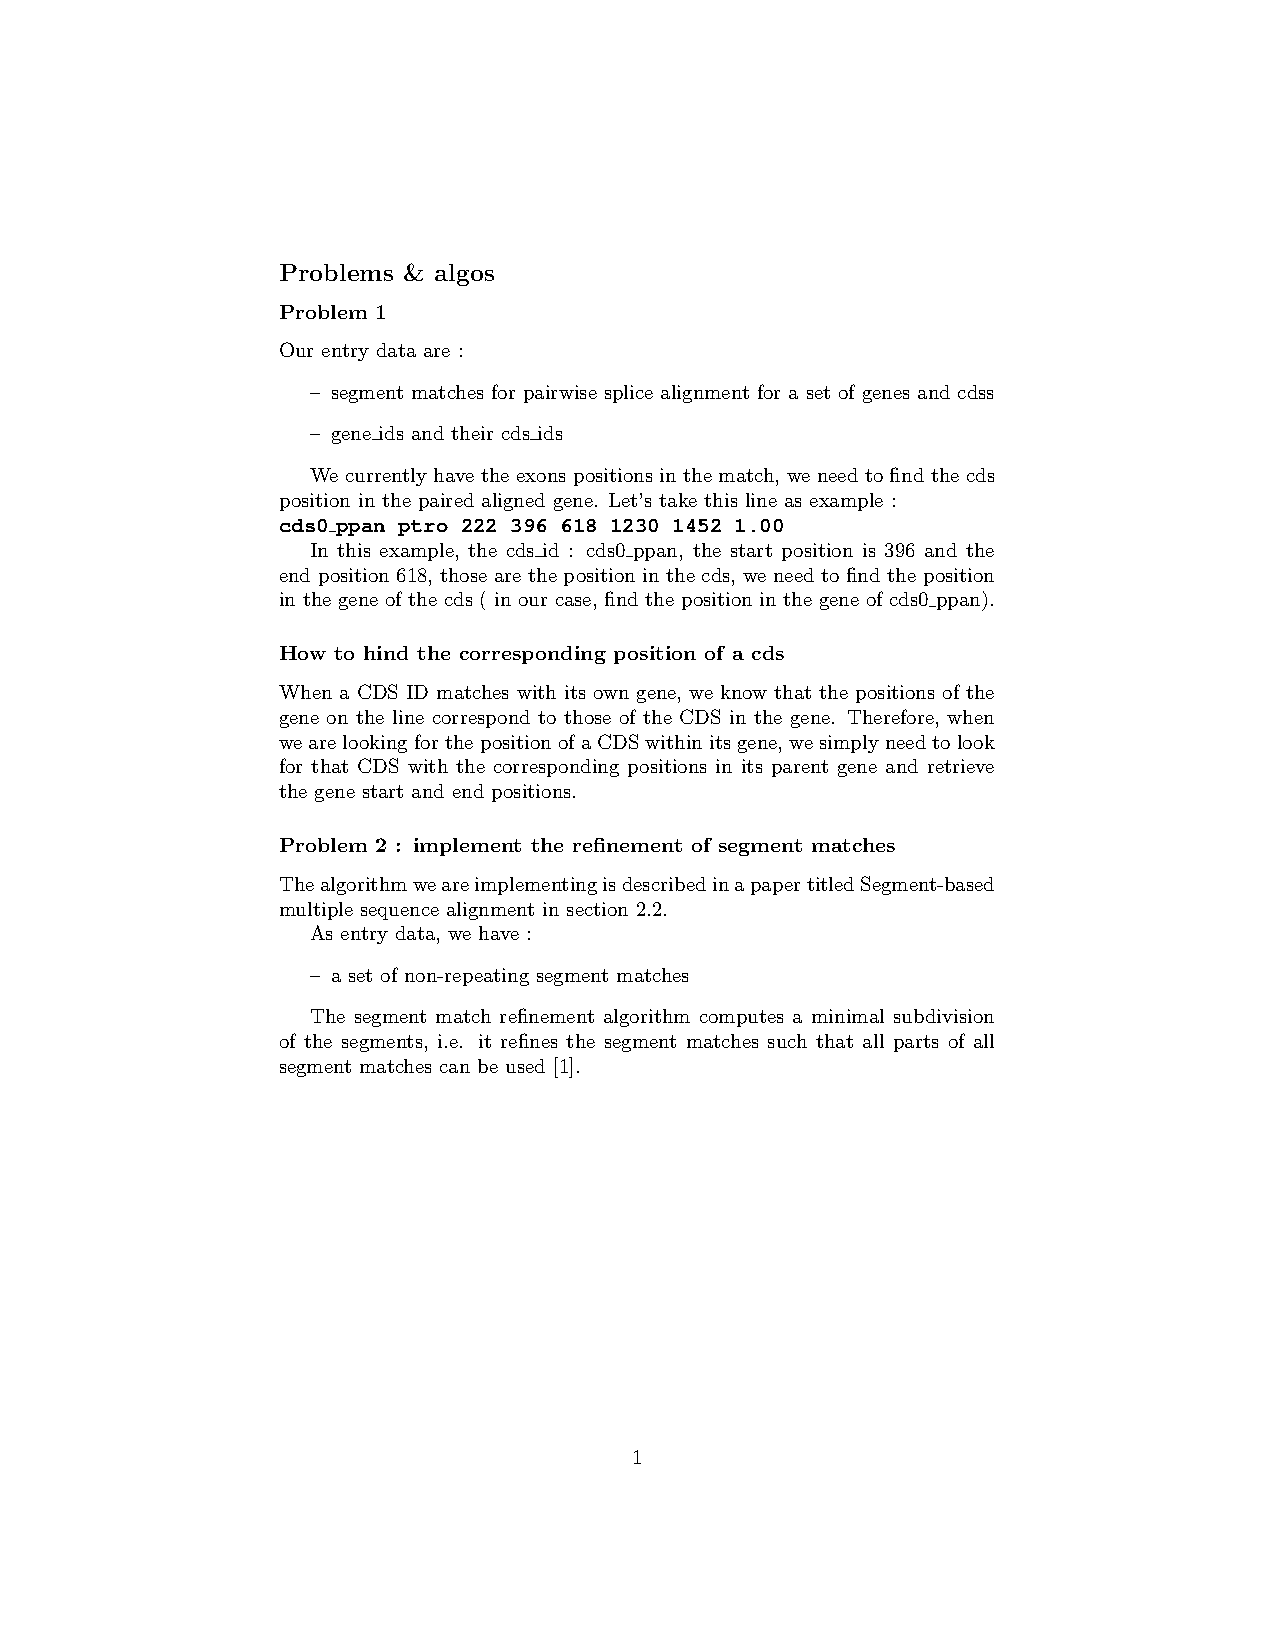
\includepdf[pages=-,scale=0.9,pagecommand={\thispagestyle{plain}}]{sources/appendix.pdf}
% % \subsection*{Problem 1}
%     Our entry data are : 
%     \begin{itemize}
%         \item[--] segment matches for pairwise splice alignment for a set of genes and cdss
%         \item[--] gene\_ids and their cds\_ids
%     \end{itemize}

%     We currently have the exons positions in the match, we need to find the cds position in the paired aligned gene. Let's take this line as example : 
    
%     \noindent\textbf{\texttt{cds0\_ppan	ptro	222	396	618	1230	1452	1.00 }}

%     In this example, the cds\_id : cds0\_ppan, the start position is 396 and the end position 618, those are the position in the cds, we need to find the position in the gene of the cds ( in our case, find the position in the gene of cds0\_ppan). 

% % \subsection*{Algo 1}
    
% \begin{algorithm}
%     \caption{Retrieve the position of the aligned exon in the other gene of the alignment}
%     \begin{algorithmic}[1]
%         \STATE \textbf{Input:} 
%         \STATE \quad $data$: segment matches for pairwise splice alignment for a set of genes and cdss
%         \STATE \quad $source\_to\_target\_file\_path$: gene\_ids and their cds\_ids
        
%         \STATE \textbf{Output:} 
%         \STATE \quad $processed$: A dictionary with additional exon position information added to the alignment data
        
%         \Procedure{FindExonPosInPairedGene}{$data, source\_to\_target\_file\_path$}
%             \STATE $cds\_gene\_map \gets \text{get\_cds\_gene\_map}(source\_to\_target\_file\_path)$
%             \STATE $result \gets \{ []\}$
            
%             \FOR{\textbf{each} $key, values$ \textbf{in} $data$}
%                 \FOR{\textbf{each} $match$ \textbf{in} $values$}
%                     \STATE $cdsId \gets match[0]$
%                     \STATE $gene_b \gets match[1]$
%                     \STATE $gene_a \gets cds\_gene\_map[cdsId]$
%                     \STATE $search\_key \gets \text{concatenate}(cdsId, gene_a)$
                    
%                     \IF{$gene_a \neq gene_b$}
%                         \STATE $result \gets \text{search\_exon\_pos\_in\_pair\_aligned\_gene}(data[search\_key], [match[3], match[4]], \text{line\_length}=10)$
                        
%                         \IF{$\text{length}(result) == 1$}
%                             \STATE \text{append}(result[0][5], result[0][6]) \text{to} match
%                             \STATE $formatted\_match \gets \text{iteration\_result\_to\_refinement\_entry\_format\_file}(match, cds\_gene\_map)$
%                             \STATE \text{append}(formatted\_match) \text{to} processed['all']
%                         \ELSE
%                             \STATE \text{append}("-", "-") \text{to} match
%                         \ENDIF
%                     \ELSE
%                         \STATE \text{append}("-", "-") \text{to} match
%                     \ENDIF
%                 \ENDFOR
%             \ENDFOR
        
%             \STATE \RETURN $processed$
%         \EndProcedure
%     \end{algorithmic}
% \end{algorithm}

% \subsection*{How to find the corresponding position of a cds}

% When a CDS ID matches with its own gene, we know that the positions of the gene on the line correspond to those of the CDS in the gene. Therefore, when we are looking for the position of a CDS within its gene, we simply need to look for that CDS with the corresponding positions in its parent gene and retrieve the gene start and end positions.


% \begin{algorithm}
%     \caption{Search Exon Positions in a Pair of Aligned Genes}
%     \begin{algorithmic}[1.1]
%         \STATE \textbf{Input:} 
%         \STATE \quad $data$: List of lines to search through
%         \STATE \quad $cds\_segment$: Tuple containing the start and end positions of the exon
%         \STATE \quad $line\_length$: Minimum length of the line to consider (default is 8)
        
%         \STATE \textbf{Output:} 
%         \STATE \quad $result$: List of lines that match the search criteria based on the exon positions
        
%         \Procedure{search\_exon\_pos\_in\_pair\_aligned\_gene}{$data, cds\_segment, line\_length=8$}
%             \STATE $(cds\_start, cds\_end) \gets cds\_segment$
%             \STATE $cds\_start \gets \text{int}(cds\_start)$
%             \STATE $cds\_end \gets \text{int}(cds\_end)$
%             \STATE $result \gets []$
            
%             \FOR{\textbf{each} $line$ \textbf{in} $data$}
%                 \IF{$( \text{int}(line[3]) == \text{exonStart} \land \text{int}(line[4]) == \text{exonEnd}) $}
%                     \STATE \text{append} $line$ \text{to} $result$
%                 \ENDIF
%             \ENDFOR

        
%             \STATE \RETURN $result$
%         \EndProcedure
%     \end{algorithmic}
% \end{algorithm}
    
% \subsection*{Problem 2 : implement the refinement of segment matches}

% The algorithm we are implementing is described in a paper titled \href{https://academic.oup.com/bioinformatics/article/24/16/i187/200409}{Segment-based multiple sequence alignment} in section 2.2.

% As entry data, we have : 
%     \begin{itemize}
%         \item[--] a set of non-repeating segment matches
%         % \item[--] 
%     \end{itemize}


% The segment match refinement algorithm computes a minimal subdivision of the segments, i.e. it refines the segment matches such that all parts of all segment matches can be used.


% \begin{algorithm}
% \caption{mult\_seg\_match\_refinement}
%     \begin{algorithmic}[2.1]
%         \REQUIRE file\_path: string
%         \ENSURE refined multi-segment matches
%         % \IF{file\_path is empty}
%         %     \PRINT{Error: File path cannot be empty}
%         %     \RETURN
%         % \ENDIF
%         % \STATE output $\gets$ \texttt{get\_output\_folder(OUTPUT\_FOLDER)} + \texttt{get\_family(file\_path).replace('\_extended\_', '')} + "\_output.txt"
%         % \STATE original\_data $\gets$ \texttt{file\_to\_list(file\_path)}
%         \STATE segment\_matches $\gets$ \texttt{original\_data[2:]}
%         \STATE Vi $\gets$ \texttt{build\_Vi(segment\_matches)}
%         \STATE \texttt{del\_duplicates\_sort\_Vi(Vi)}
%         \STATE \texttt{visualize\_Vi(Vi, output)}
%         \STATE Ti $\gets$ \texttt{build\_Ti(segment\_matches)}
%         \FORALL{match in segment\_matches}
%             % \IF{match is empty}
%             %     \CONTINUE
%             % \ENDIF
%             \STATE boundaries $\gets$ \texttt{get\_match\_boundaries(match)}
%             \FORALL{w in boundaries}
%                 \STATE gene1 $\gets$ \texttt{gene\_of\_boundary(index, match)}
%                 \STATE Vi $\gets$ \texttt{refine(w, Ti, Vi, gene1)}
%             \ENDFOR
%         \ENDFOR
%         \STATE \texttt{del\_duplicates\_sort\_Vi(Vi)}
%         \STATE \texttt{visualize\_Vi(Vi, output, True)}
%         \PRINT{Refinement output path : \texttt{output}}
%         \RETURN Vi
%     \end{algorithmic}
% \end{algorithm}

% % \begin{algorithm}
% %     \caption{refine}
% %     \begin{algorithmic}[2.2]
% %         \REQUIRE w: int, Ti: dict, Vi: dict, gene1: dict
% %         \ENSURE refined Vi
% %         \STATE overlaps $\gets$ \texttt{get\_overlaps(Ti, w, gene1["gene\_id"])}
% %         \FORALL{lq in overlaps}
% %             \STATE h $\gets$ lq.begin + (w - gene1["u"])
% %             \IF{lq.begin $<$ h $<$ lq.end}
% %                 \STATE gene2\_id $\gets$ lq.data
% %                 \STATE gene2 $\gets$ \{ "gene\_id": gene2\_id, "u": lq.begin, "v": h \}
% %                 \IF{h not in Vi[gene2\_id]}
% %                     \STATE Vi[gene2\_id].append(h)
% %                     \STATE Vi $\gets$ \texttt{refine(h, Ti, Vi, gene2)}
% %                 \ENDIF
% %             \ENDIF
% %         \ENDFOR
% %         \RETURN Vi
% %     \end{algorithmic}
% % \end{algorithm}

% \begin{algorithm}
%     \caption{refine}
%     \begin{algorithmic}[1]
%         \REQUIRE $w$, $Ti$, $Vi$, $gene1$
%         \ENSURE Refined $Vi$
%         \STATE $stack \gets [(w, gene1)]$
%         \WHILE{$stack \neq []$}
%             \STATE $(current\_w, current\_gene1) \gets stack.pop()$
%             \STATE $overlaps \gets get\_overlaps(Ti, current\_w, current\_gene1)$
%             \FORALL{$lq \in overlaps$}
%                 \IF{$lq[0].data == current\_gene1[\text{"gene\_id"}]$}
%                     \STATE $(u, v, u\_v\_gene) \gets (lq[0].begin, lq[0].end, lq[0].data)$
%                     \STATE $(x, y, x\_y\_gene) \gets (lq[1].begin, lq[1].end, lq[1].data)$
%                 \ELSE
%                     \STATE $(u, v, u\_v\_gene) \gets (lq[1].begin, lq[1].end, lq[1].data)$
%                     \STATE $(x, y, x\_y\_gene) \gets (lq[0].begin, lq[0].end, lq[0].data)$
%                 \ENDIF
%                 \STATE $h \gets x + (current\_w - u)$
%                 \STATE $gene2\_id \gets x\_y\_gene$
%                 \STATE $consider\_h \gets x < h < y$
%                 \STATE $gene2 \gets \{ \text{"gene\_id"}: gene2\_id, \text{"u"}: u, \text{"v"}: h \}$
%                 \IF{$consider\_h$}
%                     \IF{$gene2\_id \notin Vi$}
%                         \STATE $Vi[gene2\_id] \gets []$
%                     \ENDIF
%                     \IF{$h \notin Vi[gene2\_id]$}
%                         \STATE $Vi[gene2\_id].append(h)$
%                         \STATE $stack.append((h, gene2))$
%                     \ENDIF
%                 \ENDIF
%             \ENDFOR
%         \ENDWHILE
%         \STATE \RETURN $Vi$
%     \end{algorithmic}
% \end{algorithm}


% \newpage
% \subsection*{Problem 3 : alignment graph}

% The algorithm we are implementing is described in the same paper in section 2.1. The purpose of this algo is to construct an alignment graph from refined segment matches for genes. 

% \subsection*{Overall steps of the algorithm}
% \begin{enumerate}
%     \item Build vertices from the refined segments for each gene. A vertex is a tuple size 3:
%     \begin{enumerate}
%         \item[0] gene id
%         \item[1] start position
%         \item[2] length
%     \end{enumerate}
%     \item Build edges from vertices.
%     \begin{enumerate}
%         \item An edge exists if there is a match between the 2 vertices.
%         \begin{itemize}
%             \item $\diamond$ start\_i == start\_j
%             \item $\diamond$ length\_i == length\_j
%         \end{itemize}
%         \item The weight of the edge is found using the percent identity (PI) of the match represented by the edge. The triplet approach is the way:
%         \begin{enumerate}
%             \item Compute edge percent identity.
%             \item Calculate the weight (triplet approach).
%         \end{enumerate}
%     \end{enumerate}
%     \item Generate the graph using the edges.
%     \begin{itemize}
%         \item The edge structure (tuple):
%         \begin{enumerate}
%             \item[0] Vertex origin
%             \item[1] Vertex target
%             \item[2] Weight
%         \end{enumerate}
%     \end{itemize}
% \end{enumerate}

% \begin{algorithm}
%     \caption{build\_alignment\_graph}
%     \begin{algorithmic}[3.1]
%         \REQUIRE Refined segment matches for genes
%         \ENSURE Alignment graph
%         \STATE $vertices \gets build\_vertices(V_i)$
%         \STATE $edges \gets build\_edges(vertices)$
%         \FORALL{vertex \textbf{in} $vertices$}
%             \STATE Get weighted edges using vertices
%             \STATE Get trace from weighted edges
%         \ENDFOR
%         \STATE $build\_graph$
%     \end{algorithmic}
% \end{algorithm}

% \begin{algorithm}
%     \caption{build\_vertices}
%     \begin{algorithmic}[1]
%         \REQUIRE $Vi$ 
%         \ENSURE $vertices$
%         \STATE $vertices \gets []$
%         \FORALL{$(gene\_id, boundaries) \in Vi$}
%             \FOR{$index \gets 0$ \textbf{to} $len(boundaries) - 2$}
%                 \STATE $boundary \gets boundaries[index]$
%                 \STATE $next\_boundary \gets boundaries[index + 1]$
%                 \STATE $start\_boundary \gets \text{int}(boundary)$
%                 \STATE $segment\_length \gets \text{int}(next\_boundary) - start\_boundary$
%                 \STATE $vertex \gets (gene\_id, start\_boundary, segment\_length)$
%                 \STATE $vertices.append(vertex)$
%             \ENDFOR
%         \ENDFOR
%         \STATE \RETURN $vertices$
%     \end{algorithmic}
% \end{algorithm}
        
% \begin{algorithm}
%     \caption{build\_edges}
%     \begin{algorithmic}[3.2]
%         \REQUIRE $vertices$, $target\_data$
%         \ENSURE $edges$
%         \STATE $edges \gets []$
%         \STATE $weightless\_edges \gets []$
%         \FOR{$i \gets 0$ \textbf{to} $len(vertices) - 1$}
%             \STATE $vertex\_i \gets vertices[i]$
%             \STATE $vertex\_matches \gets get\_vertex\_matches(vertex\_i, vertices)$
%             \FORALL{$vertex\_j \in vertex\_matches$}
%                 \STATE $percent\_identity \gets compute\_percent\_identity(vertex\_i, vertex\_j, target\_data)$
%                 \STATE $weightless\_edges.append((vertex\_i, vertex\_j, percent\_identity))$
%             \ENDFOR
%         \ENDFOR
        
%         \FORALL{$weightless\_edge \in weightless\_edges$}
%             \STATE $(origin\_vertex, target\_vertex, percent\_identity) \gets weightless\_edge$
%             \STATE $origin\_matches \gets get\_vertex\_matches(origin\_vertex, vertices)$
%             \STATE $to\_sum \gets []$
%             \FORALL{$match \in origin\_matches$}
%                 \STATE $(gene\_id, start\_pos, length) \gets match$
%                 \IF{$gene\_id \neq target\_vertex[0]$}
%                     \STATE $triplet\_1\_pi \gets search\_edge(weightless\_edges, origin\_vertex, match)[2]$
%                     \STATE $triplet\_2\_pi \gets search\_edge(weightless\_edges, match, target\_vertex)[2]$
%                     \STATE $pi \gets \min(triplet\_1\_pi, triplet\_2\_pi)$
%                     \STATE $to\_sum.append(pi)$
%                 \ENDIF
%             \ENDFOR
%             \STATE $edge\_weight \gets \text{round}(percent\_identity + \text{sum}(to\_sum), 2)$
%             \STATE $edges.append((origin\_vertex, target\_vertex, edge\_weight))$
%         \ENDFOR
%         \STATE \RETURN $edges$
%     \end{algorithmic}
% \end{algorithm}

\label{endOfDoc}
\end{document}
